%% Copernicus Publications Manuscript Preparation Template for LaTeX Submissions
%% ---------------------------------
%% This template should be used for copernicus.cls
%% The class file and some style files are bundled in the Copernicus Latex Package which can be downloaded from the different journal webpages.
%% For further assistance please contact the Copernicus Publications at: publications@copernicus.org
%% http://publications.copernicus.org


%% Please use the following documentclass and Journal Abbreviations for Discussion Papers and Final Revised Papers.


%% 2-Column Papers and Discussion Papers
\documentclass[gmd, manuscript]{copernicus}



%% Journal Abbreviations (Please use the same for Discussion Papers and Final Revised Papers)

% Archives Animal Breeding (aab)
% Atmospheric Chemistry and Physics (acp)
% Advances in Geosciences (adgeo)
% Advances in Statistical Climatology, Meteorology and Oceanography (ascmo)
% Annales Geophysicae (angeo)
% ASTRA Proceedings (ap)
% Atmospheric Measurement Techniques (amt)
% Advances in Radio Science (ars)
% Advances in Science and Research (asr)
% Biogeosciences (bg)
% Climate of the Past (cp)
% Drinking Water Engineering and Science (dwes)
% Earth System Dynamics (esd)
% Earth Surface Dynamics (esurf)
% Earth System Science Data (essd)
% Fossil Record (fr)
% Geographica Helvetica (gh)
% Geoscientific Instrumentation, Methods and Data Systems (gi)
% Geoscientific Model Development (gmd)
% Geothermal Energy Science (gtes)
% Hydrology and Earth System Sciences (hess)
% History of Geo- and Space Sciences (hgss)
% Journal of Sensors and Sensor Systems (jsss)
% Mechanical Sciences (ms)
% Natural Hazards and Earth System Sciences (nhess)
% Nonlinear Processes in Geophysics (npg)
% Ocean Science (os)
% Proceedings of the International Association of Hydrological Sciences (piahs)
% Primate Biology (pb)
% Scientific Drilling (sd)
% SOIL (soil)
% Solid Earth (se)
% The Cryosphere (tc)
% Web Ecology (we)
% Wind Energy Science (wes)


%% \usepackage commands included in the copernicus.cls:
%\usepackage[german, english]{babel}
%\usepackage{tabularx}
%\usepackage{cancel}
%\usepackage{multirow}
%\usepackage{supertabular}
%\usepackage{algorithmic}
%\usepackage{algorithm}
%\usepackage{amsthm}
%\usepackage{float}
%\usepackage{subfig}
%\usepackage{rotating}

% Custom commands
\newcommand{\vb}{\mathbf}
\newcommand{\vg}{\boldsymbol}
\newcommand{\mat}{\mathsf}
\newcommand{\diff}[2]{\frac{d #1}{d #2}}
\newcommand{\diffsq}[2]{\frac{d^2 #1}{{d #2}^2}}
\newcommand{\pdiff}[2]{\frac{\partial #1}{\partial #2}}
\newcommand{\pdiffsq}[2]{\frac{\partial^2 #1}{{\partial #2}^2}}


\begin{document}

\title{DCMIP2016, Part 1: Models and Equation Sets}


% \Author[affil]{given_name}{surname}

\Author[1]{Paul A.}{Ullrich}
\Author[2]{Christiane}{Jablonowski}
\Author[3]{James}{Kent}
\Author[4]{Peter}{Lauritzen}
\Author[4]{Ramachandran}{Nair}
\Author[5]{Kevin A.}{Reed}
\Author[4]{Colin}{Zarzycki}

\Author[6]{Thomas}{Dubos}
\Author[7]{Marco}{Giorgetta}
\Author[8]{Elijah}{Goodfriend}
\Author[9]{David A.}{Hall}
\Author[10]{Lucas}{Harris}
\Author[8]{Hans}{Johansen}
\Author[11]{Christian}{Kuehnlein}
\Author[12]{Vivian}{Lee}
\Author[13]{Thomas}{Melvin}
\Author[14]{Hiroaki}{Miura}
\Author[15]{David}{Randall}
\Author[16]{Alex}{Reinecke}
\Author[4]{William}{Skamarock}
\Author[16]{Kevin}{Viner}
\Author[17]{Robert}{Walko}

\affil[1]{University of California, Davis}
\affil[2]{University of Michigan}
\affil[3]{University of South Wales}
\affil[4]{National Center for Atmospheric Research}
\affil[5]{Stony Brook University}
\affil[6]{Institut Pierre-Simon Laplace (IPSL)}
\affil[7]{Max Planck Institute for Meteorology}
\affil[8]{Lawrence Berkeley National Laboratory}
\affil[9]{University of Colorado, Boulder}
\affil[10]{Geophysical Fluid Dynamics Laboratory}
\affil[11]{European Center for Medium-Range Weather Forecasting}
\affil[12]{Environment Canada}
\affil[13]{U.K. Met Office}
\affil[14]{University of Tokyo}
\affil[15]{Colorado State University}
\affil[16]{Naval Research Laboratory}
\affil[17]{University of Miami}

%% The [] brackets identify the author with the corresponding affiliation. 1, 2, 3, etc. should be inserted.



\runningtitle{DCMIP2016: Models and Equation Sets}

\runningauthor{Ullrich, et al.}

\correspondence{Paul A. Ullrich (paullrich@ucdavis.edu)}



\received{}
\pubdiscuss{} %% only important for two-stage journals
\revised{}
\accepted{}
\published{}

%% These dates will be inserted by Copernicus Publications during the typesetting process.


\firstpage{1}

\maketitle



\begin{abstract}
This paper provides a comprehensive review of the design of modern non-hydrostatic atmospheric dynamical cores, including relevant equation sets, numerical stabilization techniques and idealized physics routines.
\end{abstract}



\introduction  %% \introduction[modified heading if necessary]

{\color{red}INSTRUCTIONS FOR AUTHORS}

{\color{red} Fill in text in section 3, 4, 5, 6, 7 and 8 below.}

\section{Notation}

\subsection{List of Symbols}

Table \ref{tab:symbols} lists the symbols used in this paper.

\begin{table}[h]
\caption{List of symbols used in this manuscript} \label{tab:symbols}
\begin{center}
\begin{tabular}{cl}
\hline Symbol & Description \\ \hline 
$\lambda$ & Longitude (in radians) \\
$\varphi$ & Latitude (in radians) \\
$z$ & Height with respect to mean sea level (set to zero) \\
$p_s$ & Surface pressure ($p_s$ of moist air if $q>0$) \\
$\Phi_s$ & Surface geopotential \\
$z_s$ & Surface elevation with respect to mean sea level (set to zero) \\
$u$ & Zonal wind \\
$v$ & Meridional wind \\
$w$ & Vertical velocity \\
$\omega$ & Vertical pressure velocity  \\
$\delta$ & Divergence\\
$\zeta$ & Relative vorticity\\
$p$ & Pressure (pressure of moist air if $q>0$) \\
$\rho$ & Total air density \\
$\rho_d$ & Dry air density \\
$T$ &Temperature \\
$T_v$ & Virtual temperature \\
$\Theta$ & Potential temperature \\
$\Theta_v$ & Virtual potential temperature \\
$q$ & Specific humidity \\
$P_{ls}$ & Large-scale precipitation rate \\
$q_c$ & Cloud water mixing ratio \\
$q_r$ & Rain water mixing ratio \\
\hline 
\end{tabular}
\end{center}
\end{table}

\subsection{List of Physical Constants}
A list of physical constants which are used throughout this document is given in Table \ref{tab:PhysicalConstants}.  Constants which are specific to each test case are similarly tabulated at the beginning of each section.

\begin{table}[h]
\caption{A list of physical constants used in this document.} \label{tab:PhysicalConstants}
%\ \\
\begin{tabular*}{\textwidth}{@{\extracolsep{\fill}}lll}
\hline Constant & Description & Value \\
\hline $a_{\tiny \mbox{ref}}$ & Radius of the Earth & $6.37122 \times 10^{6}\ \mbox{m}$ \\
$\Omega_{\tiny \mbox{ref}}$ & Rotational speed of the Earth & $7.292\ \times 10^{-5}\ \mbox{s}^{-1}$ \\
%$a$ & Scaled radius of the Earth & $a_{\tiny \mbox{ref}} / X$ \\
%$\Omega$ & Scaled rotational speed of the Earth & $\Omega_{\tiny \mbox{ref}} \cdot X$ \\
$g_c$ & Gravitational acceleration & $9.80616\ \mbox{m}\ \mbox{s}^{-2}$ \\
$p_0$ & Reference pressure & $1000\ \mbox{hPa}$ \\
$c_p$ & Specific heat capacity of dry air at constant pressure & $1004.5\ \mbox{J}\ \mbox{kg}^{-1}\ \mbox{K}^{-1}$ \\
$c_v$ & Specific heat capacity of dry air at constant volume & $717.5\ \mbox{J}\ \mbox{kg}^{-1}\ \mbox{K}^{-1}$ \\
$R_d$ & Gas constant for dry air & $287.0\ \mbox{J}\ \mbox{kg}^{-1}\ \mbox{K}^{-1}$ \\
$R_\nu$ & Gas constant for water vapor & $461.5$ J kg$^{-1}$ K$^{-1}$ \\
$\kappa$ & Ratio of $R_d$ to $c_p$ & $2/7$ \\
$\varepsilon$ & Ratio of $R_d$ to $R_\nu$ & $0.622$ \\
$M_v$ & Constant for virtual temperature conversion & $0.608$ \\
$\rho_{water}$ & Reference density of water & 1000 kg m$^{-3}$ \\
\hline 
\end{tabular*}

\end{table}

\subsection{Great Circle Distance}

The great circle distance is used throughout the document and is given by
\begin{equation}
R_c(\lambda_1, \varphi_1; \lambda_2, \varphi_2) = a \arccos \left( \sin \varphi_1 \sin \varphi_2 + \cos \varphi_1 \cos \varphi_2 \cos (\lambda_1 - \lambda_2) \right).
\end{equation}

%%%%%%%%%%%%%%%%%%%%%%%%%%%%%%%%%%%%%%%%%%%%%%%%%%%%%%%%%%%%%

\section{Model Grids} \label{sec:ModelGrids}

{\color{red}[ALL] Add a short description of your model grid here.}

\subsection{Yin-Yang grid} \label{sec:GEM_model_grid}
In GEM model, we use spherical coordinates on the overset Yin-Yang grid.
The Yin-Yang grid  \citep{kageama2004yinyang}  has two grid components which are geometrically
identical (see Fig. \ref{fig:gem_yinyang}). They are combined to cover a spherical surface with partial
overlap on their borders. Each component is in fact a part of the
latitude-longitude grid and is defined in spherical
polar coordinates by
\begin{equation}\label{eq:gem_yinyang}
(-\frac{\pi}{4}-\delta_{\theta} \leq \theta \leq
\frac{\pi}{4}+\delta_{\theta})  \cap
(-\frac{3\pi}{4}-\delta_{\lambda} \leq \lambda \leq
\frac{3\pi}{4}+\delta_{\lambda}),
\end{equation}
where $\delta_{\lambda}, \delta_{\theta}$ are small buffers, which are
proportional to the respective grid-spacings, required for a minimum
overlap in the overset methodology. In our DCMIP experiments, we use 
$ \delta_{\theta}=2 $ degrees and
$ \delta_{\lambda}=3 \delta_{\theta} $.
%----------------------------------------------------
\begin{figure}[]
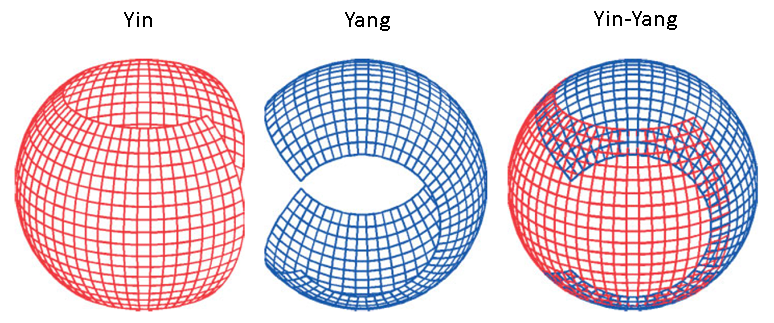
\includegraphics[height=6cm]{gem_yinyang.png}
\caption{ Yin-Yang grid }
\label{fig:gem_yinyang}
\end{figure}
%----------------------------------------------------

\subsection{Latitude-longitude grid}

\subsection{Cubed-sphere grid}

The equiangular cubed-sphere grid \citep{sadourny1972conservative, ronchi1996cubed} consists of six Cartesian patches arranged along the faces of a cube which is then inflated onto a spherical shell.  More information on this choice of grid can be found in \cite{ullrich2014global}.  On the equiangular cubed-sphere grid, coordinates are given as $(\alpha, \beta, p)$, with central angles $\alpha, \beta \in [- \frac{\pi}{4}, \frac{\pi}{4}]$ and panel index $i_p \in \{1,2,3,4,5,6\}$.  By convention, we choose panels 1--4 to be along the equator and panels $5$ and $6$ to be centered on the northern and southern pole, respectively.

\subsection{Icosahedral grid}

\subsection{Centroidal Voronoi tessellation grid}

%%%%%%%%%%%%%%%%%%%%%%%%%%%%%%%%%%%%%%%%%%%%%%%%%%%%%%%%%%%%%

\section{Equation Sets} \label{sec:EquationSets}

{\color{red}[ALL] Include the continuous equation set that you use for your model here.}

\subsection{GEM} \label{sec:GEM_equations}
The equations of GEM model \citep{Girard2014} written out for a log-hydrostatic-pressure like coordinate $\zeta$  system co-rotating with the earth are:
\begin{eqnarray}
\frac{ {d \bf V}_{h} }{dt}+ f {\bf k} \times {\bf{V}_{h}} + R_d T_v\nabla
_\zeta \,  \ln\, p+ \left( 1 + \mu \right) \nabla
_\zeta {\phi} = 0,
\label{eq:gem_eq_1} \\
\frac{d w}{dt}- g \mu = 0,
\label{eq:gem_eq_2} \\
\frac{d}{dt} \ln \left( \pi \pdiff{\ln \pi}{\zeta}\right)
+ \nabla
_{ \zeta }\cdot {\bf V}_{{h}}+\frac{\partial
\dot{ \zeta }}{\partial
\zeta }  = 0,
\label{eq:gem_eq_3} \\
\frac{d \ln T_v}{dt} - \kappa \frac {d \ln p} {dt}=0,
\label{eq:gem_eq_4} \\
R_dT_v+  \frac{p}{\pi} \frac{\partial \phi}{\partial \ln \pi}=0,
\label{eq:gem_eq_5} \\
\frac{d \phi}{dt}-  g w  = 0,
\label{eq:gem_eq_6} \\
1+ \mu - \frac{p}{\pi}   \frac{\partial \ln p}{\partial \ln  \pi}=0,
\label{eq:gem_eq_7} \\
\ln \pi= \zeta+Bs ,
\label{eq:gem_eq_8}
\end{eqnarray}

\noindent with horizontal velocity ${\bf V}_h$, 
generalized vertical velocity $\dot{ \zeta }=\frac{d\zeta}{dt}$, 
vertical velocity $w$,
geopotential $\phi$, 
virtual temperature $T_v$, 
pressure $p$ and
hydrostatic pressure $\pi$. The variable 
$\mu$ is a measure of departure from hydrostatic balance, 
$s$ is related to the surface pressure $\pi_s$ and $B$ is a metric term. The last two variables are defined in (\ref{eq:gem_zeta}).
The equations contain a total time derivative $\frac{ {d } }{dt}$ that expresses the change in time while following the air parcel.


\subsection{Tempest} \label{sec:TempestEquations}

The continuity, momentum and thermodynamic equations can be written as:
\begin{align}
\pdiff{\rho}{t} &= - \nabla \cdot (\rho \vb{u}), \\
\pdiff{\vb{u}}{t} &= - \nabla (K + \Phi) - \theta \nabla \Pi + \vg{\eta} \times \vb{u}, \\
\pdiff{\theta_v}{t} &= - \vb{u} \cdot \nabla \theta_v,
\end{align} in terms of Kinetic energy $K = \vb{u} \cdot \vb{u}$, geopotential $\Phi = g_c z$ and absolute vorticity $\vg{\eta} = \vg{\zeta} + \vg{\Omega}$, which consists of relative vorticity $\vg{\zeta} = \nabla \times \vb{u}$ and planetary vorticity $\vg{\Omega}$.  The Exner pressure is related to the prognosed density and potential temperature via
\begin{equation} \label{eq:BaseNonhydrostaticEOS}
\Pi = c_p \left( \frac{p_0}{p} \right)^{R_d/c_p} = c_p \left( \frac{R_d \rho \theta_v}{p_0} \right)^{R_d/c_v}.
\end{equation}

\subsection{Tracer transport}
In GEM model, the transport equation for tracers uses the Lagrangian form:
\begin{align}
\diff{q}{t} &= 0.
\end{align}

\vfill
\vfill

\noindent Lagrangian form:
\begin{align}
\diff{q}{t} &= 0.
\end{align}

\noindent Non-conservative Eulerian form:
\begin{align}
\pdiff{q}{t} &= - \vb{u} \cdot \nabla q.
\end{align}

\noindent Flux form:
\begin{align}
\pdiff{}{t} (\rho q) &= - \nabla \cdot (\rho q \vb{u}).
\end{align}


\subsection{Height-based coordinates}

{\color{blue}Define Unstaggered, Lorenz and Charney-Phillips staggering here}

\subsection{Mass-based coordinates} \label{sec:GEM_zeta}
The vertical coordinate of GEM model named $ \zeta$ is of a log-hydrostatic-pressure type and is defined by:
\begin{align}\label{eq:gem_zeta}
 \ln \pi= \zeta+B(\zeta) s \, \, ; \, \, B(\zeta) =\left( \frac {\zeta-\zeta_T} {\zeta_s-\zeta_T}\right)^r \,; \, s= \ln ( \frac {\pi_s} {p_{o}}) \,; \, \, p_{o}=1000 \,\, \mbox{hPa},
\end{align}
with $\zeta_T= \ln \pi_T$, $\zeta_s= \ln {p_{o}}$ and where $r$ is a variable exponent providing added freedom for adjusting the thickness of model layers over high terrain.
Figure \ref{fig:gem_charney-phillips} shows the Charney-Phillips grid in GEM model, giving the position occupied by each variable in the vertical domain.
Horizontal velocity ${\bf V}_h$, geopotential $\phi$ and $q=\ln(p/\pi)$ are on momentum levels.
Temperature $T$, vertical velocity $w$,
generalized vertical velocity $\dot{ \zeta }$ and tracers are on thermodynamic levels. 

%----------------------------------------------------
\begin{figure}[]
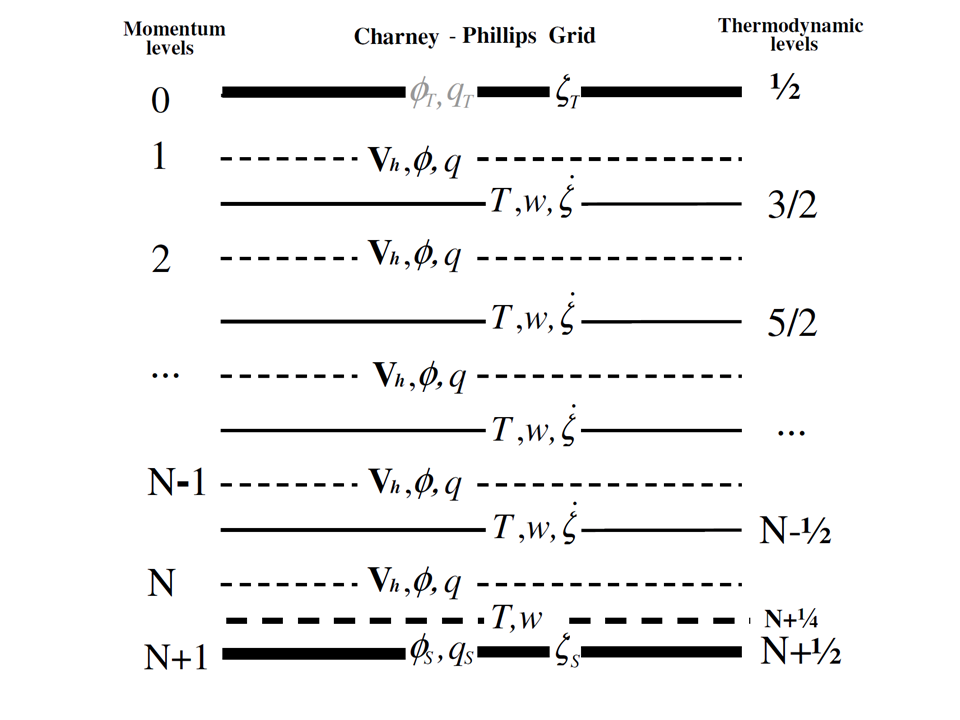
\includegraphics[height=10cm]{gem_charney-phillips.png}
\caption{ Charney-Phillips grid }
\label{fig:gem_charney-phillips}
\end{figure}
%----------------------------------------------------




%%%%%%%%%%%%%%%%%%%%%%%%%%%%%%%%%%%%%%%%%%%%%%%%%%%%%%%%%%%%%

\section{Diffusion and Stabilization} \label{sec:DiffusionStabilization}

{\color{red}[ALL] Include explicit diffusion and stabilization techniques that you have applied in the dynamical core here.}

Via an application of (\ref{eq:scalar_viscosity_direct}),
scalar viscosity is employed for wind components and tracers. 
A vertical sponge layer, also via an application of (\ref{eq:scalar_viscosity_direct}),
is employed on wind components and $T_v$ with a vertical modulation on the 6 top levels 
and a maximum damping coefficient of $.380000 \times 10^{6}\ \mbox{m\textsuperscript{2}/s}$ at the top.
For stabilization purpose, 
the temporal discretization of GEM presented  
in section \ref{sec:GEM_temporal} uses an off-centering parameter $b^{A} = 0.6$.

\subsection{Scalar viscosity}

\noindent Scalar viscosity (direct):
\begin{align} \label{eq:scalar_viscosity_direct}
\diff{s}{t} &= \ldots + \nu \nabla \cdot \nabla s.
\end{align}

\noindent Scalar viscosity (conservative):
\begin{align} \label{eq:scalar_viscosity_conservative}
\diff{}{t} (\rho q) &= \ldots + \nu \nabla \cdot ( \rho \nabla q ).
\end{align}

\subsection{Smagorinsky eddy viscosity}

\subsection{Vector viscosity, divergence and vorticity damping}

\noindent Vector viscosity:
\begin{align} \label{eq:vector_viscosity}
\diff{\vb{u}}{t} &= \ldots + \nu \nabla^2 \vb{u}
\end{align}

\noindent Divergence damping:
\begin{align} \label{eq:divergence_damping}
\diff{\vb{u}}{t} &= \ldots + \nu_{div} \nabla (\nabla \cdot \vb{u})
\end{align}

\noindent Vorticity damping:
\begin{align} \label{eq:vorticity_damping}
\diff{\vb{u}}{t} &= \ldots + \nu_{vort} \nabla \times (\nabla \times \vb{u})
\end{align}

\subsection{Hyperviscosity} \label{sec:Diffusion_Hyperviscosity}

{\color{blue}Repeated application of the scalar and vector viscosity operators}

%%%%%%%%%%%%%%%%%%%%%%%%%%%%%%%%%%%%%%%%%%%%%%%%%%%%%%%%%%%%%

\section{Filters and Fixers} \label{sec:FiltersFixers}

{\color{red}[ALL] Include explicit filters and fixers that you have utilized in the dynamical core here.}

\subsection{Mass borrowing (positive definite preservation)}
In GEM model, shape-preserving solutions are computed for tracers by using the quasi-monotone semi-Lagrangian (QMSL) method \citep{Bermejo1992QMSL}. 

\subsection{Mass fixers}

\subsection{Energy fixers}

%%%%%%%%%%%%%%%%%%%%%%%%%%%%%%%%%%%%%%%%%%%%%%%%%%%%%%%%%%%%%

\section{Temporal Discretizations} \label{sec:TemporalDiscretizations}

{\color{red}[ALL] Describe the time-stepping scheme / temporal discretization employed by your dynamical core here.}

\subsection{Runge-Kutta}

\subsubsection{Ullrich-Kinnmark-Gray 5 step 3rd order scheme} \label{sec:UKG53Scheme}

Explicit terms are evolved using a Runge-Kutta method which supports a large stability bound for spatial discretizations with purely imaginary eigenvalues. This particular scheme is based on \cite{kinnmark1984onestepA, kinnmark1984onestepB} and takes the form
\begin{align}
\psi^{(1)} &= \psi^{(0)} + \tfrac{\Delta t}{5} f(\psi^{(0)}), \nonumber \\
\psi^{(2)} &= \psi^{(0)} + \tfrac{\Delta t}{5} f(\psi^{(1)}), \nonumber \\
\psi^{(3)} &= \psi^{(0)} + \tfrac{\Delta t}{3} f(\psi^{(2)}), \\
\psi^{(4)} &= \psi^{(0)} + \tfrac{2 \Delta t}{3} f(\psi^{(3)}), \nonumber \\
\psi^{(5)} &= -\tfrac{1}{4} \psi^{(0)} + \tfrac{5}{4} \psi^{(1)} + \tfrac{3 \Delta t}{4} f(\psi^{(4)}). \nonumber
\end{align}

\subsection{Semi-Implicit time integration}

%%%%%%%%%%%%%%%%%%%%%%%%%%%%%%%%%%%%%%%%%%%%%%%%%%%%%%%%%%%%%
\subsection { The 2 time level semi-Lagrangian implicit time discretization in GEM model} \label{sec:GEM_temporal}

Consider a frictionless adiabatic prognostic equation of the form:
\begin{equation} 
\frac {dF}{dt}+G=0,
\label{eq:gem_temporal_O}
\end{equation}
\noindent where $F$ represents one of the prognostic variables and $G$ represents the remaining terms, some of which are non-linear.
Based on the semi-Lagrangian scheme,
The equation (\ref {eq:gem_temporal_O}) is discretized as:
\begin{equation} 
\frac{F^A-F^{D}} {\Delta t}+ b^A G^A + (1-b^A) G^D = 0,
\label{eq:gem_temporal_D}
\end{equation}
with $A \, \mbox{(Arrival)} = (\vg{r},t)$, $D \, \mbox{(Departure)} = (\vg{r}-\Delta \vg{r},t-\Delta t)$ 
and $\vg{r}$ is the 3D grid position. 
The displacements $\Delta \vg{r}$ are obtained by the iterative process:
\begin{equation} 
\Delta  \vg{r}^{i} =  \left [ b^A \vg{V}(\vg{r},t) + (1-b^A) \vg{V}(\vg{r}-\Delta \vg{r}^{i-1},t-\Delta t) \right ] \Delta t,
\label{eq:gem_temporal_traj} 
\end{equation} 
where  $\vg{V}$ is the 3D wind vector.
From (\ref {eq:gem_temporal_D}), we regroup unknown terms on the left-hand side 
and known terms on the right-hand side, that is:
\begin{align} 
\frac{F^A} {\tau} + G^A =  \frac{F^{D}} {\tau}- \beta G ^{D}= R,
\label{eq:gem_temporal_AD}
\end{align}
\noindent where $\tau= \Delta t b^A$ and $\beta = (1-b^A)/b^A$. 
Cubic Lagrange interpolation is used for upstream evaluations $(F^{D}, G^{D})$.
Each left-hand side term $\frac{F^A} {\tau}+ G^A$ is then split into a linear part $L$ and a nonlinear residual part $N$:   
\begin{align} 
\frac{F^A} {\tau} + G^A = L + N = R. 
\label{eq:gem_temporal_LN}
\end{align}
The linearization is done around a constant in time, horizontally homogeneous, reference state. 
This results in the non-linear problem:
\begin{align}
L^{i}=R-N^{i-1},
\label{eq:gem_temporal_solve}
\end{align}
which is solved with two iterations.   
In each iteration, the
linear system (\ref{eq:gem_temporal_solve})  
is reduced to an Helmholtz problem 
for one composite variable.
It 
is solved 
with a direct solver
using the Schwarz-type domain decomposition method on Yin-Yang grid \citep{Qaddouri2008schwarz}.
The composite variable solution is used to update the prognostic variables at time $t$.  
Our procedure involves another iterative process linked to the estimation of $\vg{V}(\vg{r},t)$ in the displacement calculations (\ref{eq:gem_temporal_traj}). 
This results in redoing the sequence of operations (\ref{eq:gem_temporal_traj})-(\ref{eq:gem_temporal_solve}). 
At each time step, the cubic Lagrange interpolation is used to update the static halo region of both panels of the Yin-Yang grid 
\citep{Qaddouri2011operational}. 

\section{Dynamical Cores}

{\color{red}In this section provide a short description (approximately 0.5 pages) of the dynamical core, focusing on unique features or design specifications.  Do not include information on the physical parameterizations used by the modeling system.  Make reference to the model grid employed from section \ref{sec:ModelGrids}, the specific equation set being discretized by the model in section \ref{sec:EquationSets}, explicit numerical techniques for diffusion and stabilization in section \ref{sec:DiffusionStabilization}, filters and fixers in section \ref{sec:FiltersFixers} and the temporal discretization in section \ref{sec:TemporalDiscretizations}.}

\subsection{Tempest}

{\color{red}[ULLRICH]}

The Tempest model \citep{ullrich2014global, guerra2016high} uses a horizontal spectral element discretization and vertical staggered nodal finite element method based on the cubed-sphere grid with terrain-following height-based coordinate.  The standard Eulerian equations are employed with moist density $\rho$, thermodynamic closure $\theta_v$ and tracer density $\rho q$.  These continuous equations are given in section \ref{sec:TempestEquations}.  The implementation includes both fully explicit time integration, using the UKG53 scheme described in section \ref{sec:UKG53Scheme}, and implicit-explicit options, where horizontal terms are explicitly discretized and vertical terms are treated implicitly.  Scalar hyperviscosity is employed for $\rho$, $\theta$ and tracer variables via repeated application of (\ref{eq:scalar_viscosity_direct}).  Vector hyperviscosity is also applied by decomposing the horizontal vector Laplacian into divergence damping (\ref{eq:divergence_damping}) and vorticity damping (\ref{eq:vorticity_damping}) terms.  Both viscosity operations are applied after the completion of all Runge-Kutta sub-cycles.

\subsection{High-Order Method Modeling Environment (HOMME)}

{\color{red}[HALL]}

\subsection{Model for Prediction Across Scales (MPAS)}

{\color{red}[SKAMAROCK]}

\subsection{Colorado State University Model (CSU)}

{\color{red}[RANDALL]}

\subsection{Geophysical Fluid Dynamics Laboratory FV Cubed (GFDL-FV3)}

{\color{red}[HARRIS]}

\subsection{Chombo}

{\color{red}[JOHANSEN]}

\subsection{Naval Research Laboratory NEPTUNE Model}

{\color{red}[VINER, REINECKE]}

\subsection{Global Environmental Multiscale (GEM) Model} \label{sec:GEM_core}

In GEM model, we use the Yin-Yang grid and horizontal discretization is done on an Arakawa C grid.
The vertical coordinate $\zeta$ is of a log-hydrostatic-pressure type and vertical discretization is based  
on the Charney-Phillips grid.
A 2 time level semi-Lagrangian implicit time discretization is implemented as described in section \ref{sec:GEM_temporal}. 
A scalar viscosity is employed for wind components and tracers 
via an application of (\ref{eq:scalar_viscosity_direct}). 
Viscosity operations are applied after the completion of the dynamic time step.

\subsection{Ocean-Land-Atmosphere Model (OLAM)}

{\color{red}[WALKO]}

\subsection{DYNAMICO}

{\color{red}[DUBOS]}

\subsection{ECMWF PentaRei Finite Volume Model}

{\color{red}[KUEHNLEIN]}

\subsection{Icosahedral Non-hydrostatic (ICON) Model}

{\color{red}[GIORGETTA]}

\subsection{Nonhydrostatic ICosahedral Atmospheric Model (NICAM) Model}

{\color{red}[MIURA]}

%%%%%%%%%%%%%%%%%%%%%%%%%%%%%%%%%%%%%%%%%%%%%%%%%%%%%%%%%%%%%

\section{Idealized Physical Parameterizations}

\subsection{Kessler Physics} \label{sec:KesslerPhysics}

The cloud microphysics update according to the following equation set:
\begin{alignat}{5}
\frac{\Delta \theta}{\Delta t} = & - \frac{L}{c_p \pi} & \Big( \frac{\Delta q_{vs}}{\Delta t} & + E_r  \Big) & \\
\frac{\Delta q_v}{\Delta t} = & & \frac{\Delta q_{vs}}{\Delta t} & + E_r \\
\frac{\Delta q_c}{\Delta t} = & & - \frac{\Delta q_{vs}}{\Delta t} & & - A_r & - C_r \\
\frac{\Delta q_r}{\Delta t} = & & & - E_r & + A_r & + C_r & - V_r \pdiff{q_r}{z},
\end{alignat} where $L$ is the latent heat of condensation, $A_r$ is the autoconversion rate of cloud water to rain water, $C_r$ is the collection rate of rain water, $E_r$ is the rain water evaporation rate, and $V_r$ is the rain water terminal velocity.

The pressure follows from the equation of state
\begin{equation}
p=\rho R_dT(1+0.61q_v)
\end{equation} with $p$ the pressure, $\rho$ the density of moist air, $R_d$ the gas constant for dry air, $T$ the temperature and $q_v$ the mixing ratio of water vapor. The equation is rewritten as a nondimensional pressure $\Pi$ equation.
\begin{equation}
\pi = \left(\frac{p}{p_0}\right)^{\frac{R_dT}{cp}}
\end{equation}

To determine the saturation vapor mixing ratio the Teten's formula is used,
\begin{equation}
q_{vs}(p,T) = \left( \frac{380.0}{p} \right) \exp\left(17.27 \times \frac{T-273.0}{T-36.0}\right)
\end {equation}

The autoconvection rate ($A_r$) and collection rate ($C_r$) follow Kessler parametrization and are defined by:
\begin{align}
A_r &= k_1(q_c-a) \\
C_r &= k_2q_cq_r^{0.875}
\end{align} With $k_1=0.001 \text{s}^{-1}$, $a=0.001 \text{g}.\text{g}^{-1}$ and $k_2=2.2 \text{s}^{-1}$ 

Deriving from \cite{klemp1978simulation} description of cloud water,rain water and water vapor mixing ratios. they are define as followed:
\begin{equation}
q_c^{n+1}=\mbox{max}(q_c^r-\Delta q_r,0)
\end{equation}
\begin{equation}
q_r^{n+1}=\mbox{max}(q_r^r-\Delta q_r+S,0)
\end{equation} where $S$ is the sedimentation term and $\Delta q_r$ is defined as
\begin{equation}
\Delta q_r=q_c^n-\frac{q_c^n-\Delta \text{t}\ \mbox{max}(A_r,0)}{1+\Delta \text{t} C_r}
\end{equation}

The Rain evaporation equation is defined similarly to \cite{ogura1971numerical} description:
\begin{equation}
E_r=\frac{1}{\rho}\frac{\left(1-\frac{q_v}{q_{vs}}\right)C(\rho q_r)^{0.525}}{5.4\times10^5+\frac{2.55\times10^6}{pq_{vs}}}
\end{equation}  With ventilation factor C define as 
\begin{equation}
C_r=1.6+124.9(\rho q_r)^{0.2046}
\label{venti}
\end{equation}

The liquid water terminal velocity is similar to \cite{soong1973comparison} description with a mean density adjustment as suggested by \cite{kessler1969distribution}:
\begin{equation}
V_r = 36349(\rho q_r)^{0.1346}\left(\frac{\rho}{\rho_0}\right)^{-\frac{1}{2}}
\end{equation}

%%%%%%%%%%%%%%%%%%%%%%%%%%%%%%%%%%%%%%%%%%%%%%%%%%%%%%%%%%%%%

\subsection{Simplified Mixing in the Planetary Boundary Layer} \label{sec:PlanetaryBoundaryLayer}

The forcing by the planetary boundary layer is described in \cite{reed2012idealized} and is partly reproduced here.  To parameterize the surface fluxes that impact the zonal velocity $u$, the meridional velocity $v$ and moisture $q$ we start with the time rate of change equations
\begin{eqnarray}
\frac{\partial u}{\partial t} &=& - \frac{1}{\rho} \frac{\partial \rho \ \overline{w'u'}}{\partial z} \label{eqturb}  \\
\frac{\partial v}{\partial t} &=& - \frac{1}{\rho} \frac{\partial \rho \ \overline{w'v'}}{\partial z}  \label{eqturb_v} \\
\frac{\partial q}{\partial t} &=& - \frac{1}{\rho} \frac{\partial \rho \ \overline{w'q'}}{\partial z}.  \label{eqturb_last}
\end{eqnarray}  Potential temperature, as opposed to temperature, is used in the boundary layer parameterization because the vertical profile of the potential temperature is a suitable indicator of static stability.  This adds the time rate of change equation
\begin{eqnarray}
\frac{\partial \Theta}{\partial t} &=& - \frac{1}{\rho} \frac{\partial \rho \ \overline{w'\Theta'}}{\partial z}.
\end{eqnarray}  Here $u'$, $v'$, $w'$, $\Theta'$ and $q'$ symbolize the deviations of the zonal velocity, meridional velocity, vertical velocity, potential temperature and specific humidity from their averages, respectively. The average is indicated by an overbar.  Note, assuming pressure is held constant (which is a common assumption in physical parameterizations), the potential temperature time tendency can be converted back to a temperature tendency of the following form
\begin{eqnarray}
\frac{\partial T}{\partial t} &=& - \frac{1}{\rho} \left (\frac{p}{p_0} \right )^{\kappa} \frac{\partial \rho \ \overline{w'\Theta'}}{\partial z}.
\end{eqnarray}
with the reference pressure $p_0 = 1000$ hPa.

The turbulent mixing is characterized by a constant vertical eddy diffusivity to represent Ekman-like profiles of boundary layers
\begin{eqnarray}\label{ktheory}
\overline{w'u'} = -K_m \frac{\partial u}{\partial z} \\
\overline{w'v'} = -K_m \frac{\partial v}{\partial z} \\
\overline{w'\Theta'} = -K_E \frac{\partial \Theta}{\partial z} \\
\overline{w'q'} = -K_E \frac{\partial q}{\partial z}. 
\end{eqnarray}
Here, $K_m$ is the eddy diffusivity coefficient for momentum and $K_E$ is the eddy diffusivity coefficient for energy and set equal to that for water vapor. In order to calculate the eddy diffusivity coefficients, the eddy diffusivity is matched to that for the surface flux calculated in Appendix~\ref{sec:OceanSurfaceFluxes} at the lowermost model level.  To allow for a smooth transition above the boundary layer ($p_{top} = 850$ hPa)  the diffusivity coefficients for momentum taper to zero as
\begin{equation} \label{Kmtaper}
\begin{array}{ll}
K_m = C_d \vert \vec{v}_{a} \vert z_a & \mbox{for} \; p > p_{top} \\
K_m = C_d \vert \vec{v}_{a} \vert z_a \exp \left ( -\left [ \frac{p_{top} - p}{p_{strato}} \right ]^2 \right ) & \mbox{for} \; p \leq p_{top}.
\end{array}
\end{equation}
Here the constant $p_{strato}$ determines the rate of decrease and is set to 100 hPa. $K_E$ is defined by
\begin{equation}
\begin{array}{ll}\label{KEtaper}
K_E = C_E \vert \vec{v}_{a} \vert z_a & \mbox{for} \; p > p_{top} \\
K_E = C_E \vert \vec{v}_{a} \vert z_a \exp \left ( -\left [ \frac{p_{top} - p}{p_{strato}} \right ]^2 \right ) & \mbox{for} \; p \leq p_{top}.
\end{array}
\end{equation}
We suggest implementing the boundary layer scheme with an implicit temporal discretization to avoid numerical instabilities. The details of this discretization are somewhat complicated, and so we refer to implementation details in Appendix D of \cite{reed2012idealized}. In addition, we supply the DCMIP modeling groups with the complete ``simple-physics'' package as used in the model CAM which can serve as a template routine.

\conclusions  %% \conclusions[modified heading if necessary]
TEXT




%\appendix
%\section{}    %% Appendix A

%\subsection{}                               %% Appendix A1, A2, etc.


\authorcontribution{TEXT}

\begin{acknowledgements}
{\color{blue}[Include a complete list of DCMIP2016 student participants here along with sponsors]}
\end{acknowledgements}


%% REFERENCES

%% Since the Copernicus LaTeX package includes the BibTeX style file copernicus.bst,
%% authors experienced with BibTeX only have to include the following two lines:
%%
\bibliographystyle{copernicus}
\bibliography{DCMIP2016.bib}
%%
%% URLs and DOIs can be entered in your BibTeX file as:
%%
%% URL = {http://www.xyz.org/~jones/idx_g.htm}
%% DOI = {10.5194/xyz}


%% LITERATURE CITATIONS
%%
%% command                        & example result
%% \citet{jones90}|               & Jones et al. (1990)
%% \citep{jones90}|               & (Jones et al., 1990)
%% \citep{jones90,jones93}|       & (Jones et al., 1990, 1993)
%% \citep[p.~32]{jones90}|        & (Jones et al., 1990, p.~32)
%% \citep[e.g.,][]{jones90}|      & (e.g., Jones et al., 1990)
%% \citep[e.g.,][p.~32]{jones90}| & (e.g., Jones et al., 1990, p.~32)
%% \citeauthor{jones90}|          & Jones et al.
%% \citeyear{jones90}|            & 1990



%% FIGURES

%% ONE-COLUMN FIGURES

%%f
%\begin{figure}[t]
%\includegraphics[width=8.3cm]{FILE NAME}
%\caption{TEXT}
%\end{figure}
%
%%% TWO-COLUMN FIGURES
%
%%f
%\begin{figure*}[t]
%\includegraphics[width=12cm]{FILE NAME}
%\caption{TEXT}
%\end{figure*}
%
%
%%% TABLES
%%%
%%% The different columns must be seperated with a & command and should
%%% end with \\ to identify the column brake.
%
%%% ONE-COLUMN TABLE
%
%%t
%\begin{table}[t]
%\caption{TEXT}
%\begin{tabular}{column = lcr}
%\tophline
%
%\middlehline
%
%\bottomhline
%\end{tabular}
%\belowtable{} % Table Footnotes
%\end{table}
%
%%% TWO-COLUMN TABLE
%
%%t
%\begin{table*}[t]
%\caption{TEXT}
%\begin{tabular}{column = lcr}
%\tophline
%
%\middlehline
%
%\bottomhline
%\end{tabular}
%\belowtable{} % Table Footnotes
%\end{table*}
%
%
%%% NUMBERING OF FIGURES AND TABLES
%%%
%%% If figures and tables must be numbered 1a, 1b, etc. the following command
%%% should be inserted before the begin{} command.
%
%\addtocounter{figure}{-1}\renewcommand{\thefigure}{\arabic{figure}a}
%
%
%%% MATHEMATICAL EXPRESSIONS
%
%%% All papers typeset by Copernicus Publications follow the math typesetting regulations
%%% given by the IUPAC Green Book (IUPAC: Quantities, Units and Symbols in Physical Chemistry,
%%% 2nd Edn., Blackwell Science, available at: http://old.iupac.org/publications/books/gbook/green_book_2ed.pdf, 1993).
%%%
%%% Physical quantities/variables are typeset in italic font (t for time, T for Temperature)
%%% Indices which are not defined are typeset in italic font (x, y, z, a, b, c)
%%% Items/objects which are defined are typeset in roman font (Car A, Car B)
%%% Descriptions/specifications which are defined by itself are typeset in roman font (abs, rel, ref, tot, net, ice)
%%% Abbreviations from 2 letters are typeset in roman font (RH, LAI)
%%% Vectors are identified in bold italic font using \vec{x}
%%% Matrices are identified in bold roman font
%%% Multiplication signs are typeset using the LaTeX commands \times (for vector products, grids, and exponential notations) or \cdot
%%% The character * should not be applied as mutliplication sign
%
%
%%% EQUATIONS
%
%%% Single-row equation
%
%\begin{equation}
%
%\end{equation}
%
%%% Multiline equation
%
%\begin{align}
%& 3 + 5 = 8\\
%& 3 + 5 = 8\\
%& 3 + 5 = 8
%\end{align}
%
%
%%% MATRICES
%
%\begin{matrix}
%x & y & z\\
%x & y & z\\
%x & y & z\\
%\end{matrix}
%
%
%%% ALGORITHM
%
%\begin{algorithm}
%\caption{�}
%\label{a1}
%\begin{algorithmic}
%�
%\end{algorithmic}
%\end{algorithm}
%
%
%%% CHEMICAL FORMULAS AND REACTIONS
%
%%% For formulas embedded in the text, please use \chem{}
%
%%% The reaction environment creates labels including the letter R, i.e. (R1), (R2), etc.
%
%\begin{reaction}
%%% \rightarrow should be used for normal (one-way) chemical reactions
%%% \rightleftharpoons should be used for equilibria
%%% \leftrightarrow should be used for resonance structures
%\end{reaction}
%
%
%%% PHYSICAL UNITS
%%%
%%% Please use \unit{} and apply the exponential notation


\end{document}
